\documentclass{article}
\usepackage{graphicx} % Required for inserting images
\usepackage{amsmath}
\usepackage[margins = 1in]{geometry}
\usepackage{float}
\usepackage{hyperref}
\usepackage{xcolor}
\title{Assignment 4}
\author{Ojas Phadake ch22b007}

\begin{document}

\maketitle
\begin{center}
{Username : \href{https://github.com/ojasph}{ojasph} }
\end{center}
{\Huge\begin{center}
    Apollonius Theorem
      \end{center}} 

\section{Introdution}
\textbf{Apollonius's Theorem} relates the length of  a median with the length of it's sides. 

Say for a triangle $\Delta$ABC. And let a median be drawn from A to the opposite side, at D. The sum of the squares of the two sides, i.e. AB and AC are equal to twice the sum of the squares AM and BM. 

So, 
\begin{equation}
    |AB|^2 + |AC|^2 = 2(|AD|^2 + |BM|^2)
\end{equation}

It can also be restated as 
\begin{equation}
    2(|AB|^2 + |AC|^2) = |BC|^2 + 4|AM|^2
\end{equation}

It is a special form of Stewart's theorem, and is also called as Extended Pythagoras Theorem. For an isosceles triangle, the theorem reduces to Pythagorean theorem for the smaller triangle. 

The theorem is named for the ancient Greek mathematician Apollonius of Perga.

\begin{figure}[H]
    \centering
    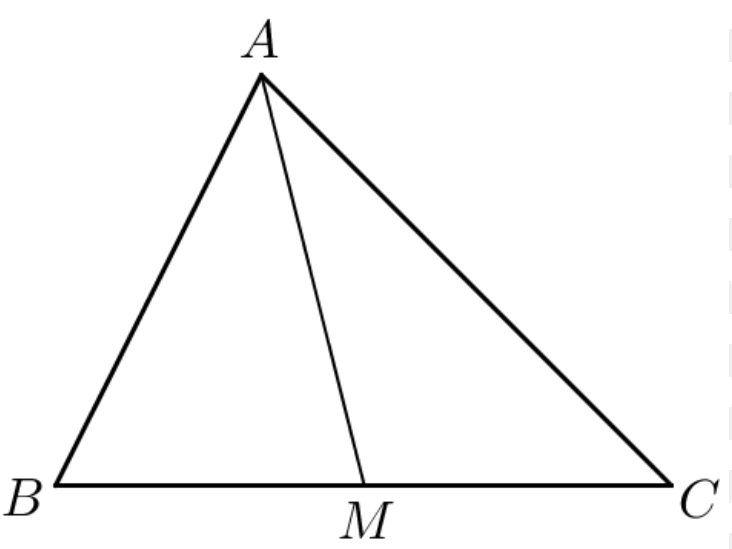
\includegraphics[width = 5cm]{Screenshot 2023-06-13 235751.png}
    \caption{Figure of the above explanation}
\end{figure}

\footnote
{\href{https://en.wikipedia.org/wiki/Apollonius\%27s\_theorem}{\textcolor{blue}{Wikipedia article on Apollonius Theorem}}}
\end{document}